\documentclass[usenames,dvipsnames]{beamer}



% For more themes, color themes and font themes, see:
% http://deic.uab.es/~iblanes/beamer_gallery/index_by_theme.html
%
\mode<presentation>
{
  \usetheme{Madrid}       % or try default, Darmstadt, Warsaw, ...
  \usecolortheme{seagull} % or try albatross, beaver, crane, ...
  \usefonttheme{default}    % or try default, structurebold, ...
  \setbeamertemplate{navigation symbols}{}
  \setbeamertemplate{caption}[numbered]
} 



\newcommand\pro{\item[$+$]}
\newcommand\con{\item[$-$]}

\usepackage{xcolor}
\usepackage{hyperref}
\usepackage{amsmath}
\usepackage[english]{babel}
\usepackage[utf8x]{inputenc}

\usepackage{listings}

\lstset{
  commentstyle=\color{ForestGreen},
  backgroundcolor=\color{white},   % choose the background color; you must add \usepackage{color} or \usepackage{xcolor}; should come as last argument
  basicstyle=\ttfamily\scriptsize,        % the size of the fonts that are used for the code
  breakatwhitespace=false,         % sets if automatic breaks should only happen at whitespace
  breaklines=true,                 % sets automatic line breaking
  captionpos=b,                    % sets the caption-position to bottom
  deletekeywords={...},            % if you want to delete keywords from the given language
  escapeinside={\%*}{*)},          % if you want to add LaTeX within your code
  extendedchars=true,              % lets you use non-ASCII characters; for 8-bits encodings only, does not work with UTF-8
  frame=single,	                   % adds a frame around the code
  keepspaces=true,                 % keeps spaces in text, useful for keeping indentation of code (possibly needs columns=flexible)
  keywordstyle=\color{blue},       % keyword style
  language=java,                 % the language of the code
  morekeywords={contract, uint, constructor, function, pragma, solidity, *},            % if you want to add more keywords to the set
  numbers=left,                    % where to put the line-numbers; possible values are (none, left, right)
  numbersep=5pt,                   % how far the line-numbers are from the code
  numberstyle=\tiny\color{gray}, % the style that is used for the line-numbers
  rulecolor=\color{black},         % if not set, the frame-color may be changed on line-breaks within not-black text (e.g. comments (green here))
  showspaces=false,                % show spaces everywhere adding particular underscores; it overrides 'showstringspaces'
  showstringspaces=false,          % underline spaces within strings only
  showtabs=false,                  % show tabs within strings adding particular underscores
  stepnumber=2,                    % the step between two line-numbers. If it's 1, each line will be numbered
  stringstyle=\color{orange},     % string literal style
  tabsize=2,	                   % sets default tabsize to 2 spaces
  title=\lstname                   % show the filename of files included with \lstinputlisting; also try caption instead of title
}

\setlength\itemsep{2em}

% adapted from https://tex.stackexchange.com/questions/89574/language-option-supported-in-listings
\lstdefinelanguage{Solidity}{
	keywords={typeof, new, true, false, catch, function, return, null, catch, 
		switch, var, if, in, while, do, else, case, break, uint8, public, 
		private, internal, external, view, 	returns, emit, require, pragma,
		solidity, contract, address, event,	modifier, constructor},
	keywordstyle=\color{blue}\bfseries,
	ndkeywords={class, export, boolean, throw, implements, import, this},
	ndkeywordstyle=\color{darkgray}\bfseries,
	identifierstyle=\color{black},
	sensitive=false,
	comment=[l]{//},
	morecomment=[s]{/*}{*/},
	commentstyle=\color{purple}\ttfamily,
	stringstyle=\color{orange}\ttfamily,
	morestring=[b]',
	morestring=[b]"
}




% Here's where the presentation starts, with the info for the title slide
\title{Ethereum}
\subtitle{Introduction and overview of existing verification procedures}
\author{Mirko Bez}
\institute{Università di Padova}
\date{\today}

\begin{document}

\begin{frame}
  \titlepage
\end{frame}

\begin{frame}{Verification Motivation}
\begin{itemize}
\item Smart contracts can manage a lot of money
\item The DAO attack costed around $60$\$ milion dollars
\begin{itemize}
\item Exploits re-entrancy vulnerability
\item Separation of the community: Ethereum Classic vs Ethereum
\end{itemize}
\end{itemize}

\begin{figure}
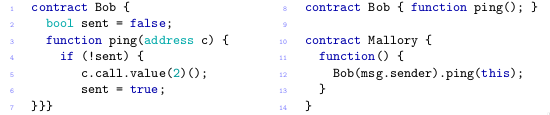
\includegraphics[width=0.9\textwidth]{./img/reentrancy}
\end{figure}

\begin{itemize}
\item Parity multiwallet signature
\begin{itemize}
\item Attackers "accidentally" \textbf{froze} $300$\$ milion dollars
\end{itemize}
\end{itemize}

\end{frame}

\begin{frame}{Common Bugs/Vulnerabilities}
\framesubtitle{\cite{bib:atzei,luu2016making}}
The majority of bugs are due to erroneous assumptions on the semantics of the EVM by developers
\begin{itemize}
\item Call to unknown
\item Mishandled Exception
\item Reentrancy
\item Transaction-ordering dependence (TOD)
\item Timestamp dependence
\item etc.
\end{itemize}

\end{frame}


\begin{frame}{Object of Verification}

\begin{block}{EVM}
\begin{itemize}
\pro It is stored on the blockchain
\pro gas consumption defined only for bytecode
\con Developers do not read bytecode
\end{itemize}
\end{block}

\begin{block}{Intermediate Language}
\begin{itemize}
\pro more high-level than bytecode
\con closer to bytecode wrt high-level language
\end{itemize}
\end{block}

\begin{block}{Solidity}
\begin{itemize}
\con Source code not necessarily public
\con Solidity change rapidly (still not 1.0)
\con Lack of formal specification
\pro Code readable by developers and auditors
\end{itemize}
\end{block}

\end{frame}





\begin{frame}{Theorem Provers}
    \begin{block}{\cite{hirai2017defining}}
        \begin{itemize}
            \item Definition of (part of) EVM in Lem
            \item Use Isabelle/HOL to proof invariants in 
            contracts
        \end{itemize}
    \end{block}
    \begin{block}{\cite{towardsVerifyingEthereumSmartContract}}
        \begin{itemize}
            \item Extension of Hirai's EVM definiton
            \item Verification against \textbf{stdandard test suites}
            \item Build CFG (identify basic blocks):
            \item Define rules for programs, basic blocks and instructions  
            \item Separation logic ($\vDash\ [P]\ c\ [Q]$)
            \item Write manually the specification
            \item Prove theorems by using Isabelle/HOL
        \end{itemize}
    \end{block}

\end{frame}



\begin{frame}{Making smart contract smarter}
\framesubtitle{\cite{luu2016making}}

\begin{itemize}
\item Describe security bugs in smart contract development:
\begin{itemize}
\item Transaction-ordering dependence (TOD)
\item Timestamp dependence
\item Mishandled exception
\item Reentrancy vulnerability
\item A survey on vulnerabilities and attacks~\cite{bib:atzei}
\end{itemize}
\item Recommendations for Better Semantics
\begin{itemize}
\item Guarded Transactions: add premise $\sigma \vdash g$
\item Prefer \texttt{block.number} to \texttt{block.timestamp}
\item Better Exception Handling
\end{itemize}


\item Formalized operational semantics:
\begin{itemize}
\item Formation and Validation of blocks
\item Transaction Execution
\item EtherLite: formalization of the EVM instructions
\end{itemize}
\end{itemize}

\end{frame}

\begin{frame}{Making smart contract smarter}
\framesubtitle{\cite{luu2016making}}
\begin{itemize}
\item Architecture of \textbf{OYENTE}:
%\item Since the proposed update require that \emph{all} clients update
\end{itemize}
\begin{center}
	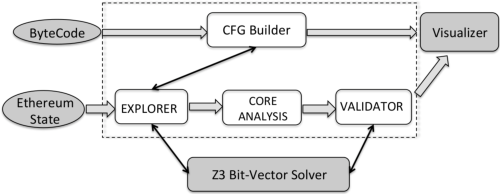
\includegraphics[width=\textwidth]{./img/oyente-architecture.pdf}
\end{center}
\end{frame}

\begin{frame}{Oyente Drawbacks}
\framesubtitle{\cite{grishchenko2018semantic,bib:securify}}
\begin{itemize}
\item Luu et al., considers only a variation of a subset of EVM bytecode: e.g. do not consider CREATE instruction
\item Some checks are neither sound nor complete (e.g. ISZERO check)
\item Conceptual flow: 
\begin{itemize}
\item global state non-included in the activation records of the call stack
\end{itemize}
\item False positives and false negatives
\end{itemize}

\end{frame}


\begin{frame}{ETHIR}
\framesubtitle{\cite{bib:vyper-docs}}
	\begin{itemize}
		\item Decompilation of EVM bytecode
		\item Modify Oyente to generate whole CFG
		\begin{itemize}
			\item If Solidity code available add information (e.g. function
			name)
		\end{itemize}
		\item Translation of bytecode into Rule-Based Representation (RBR)
		\item Analyze quantitative properties by using the high-level analyzer
		SACO~\cite{bib:SACO}:
		\begin{itemize}
			\item Upper bound on number of iterations
			\item Useful to infer gas consumptions
		\end{itemize}
		\item It is possible to adapt other static analyzers that work on
		Intermediate Representation (e.g. AproVe, T2, VeryMax, CoFloCo)
	\end{itemize}
\end{frame}



\begin{frame}{EVM rigorous semantics}

    \begin{block}{\cite{grishchenko2018semantic}}
        \begin{itemize}
            \item Rigorous complete small-step semantics of EVM bytecode
            \item Implementation of the semantics in F*
            \begin{itemize}
                \item Dialect of ML can be compiled in OCaml
                \item Validation against standard test suite
            \end{itemize}
            \item Allows definition and check of security definitions, based on
            execution traces:
            \begin{itemize}
                \item Call Integrity
                \item Exception Handling
            \end{itemize}
            \item Base work for EtherTrust
        \end{itemize}
    \end{block}

    \begin{block}{KEVM~\cite{bib:kevm}}
        \begin{itemize}
            \item Definition of EVM with $\mathbb{K}$-Framework
            \item Show properties with reachability logic
        \end{itemize}
    \end{block}

\end{frame}





\begin{frame}{Formal Verification of Smart Contract}
\framesubtitle{\cite{bhargavan2016formal}}
\begin{center}
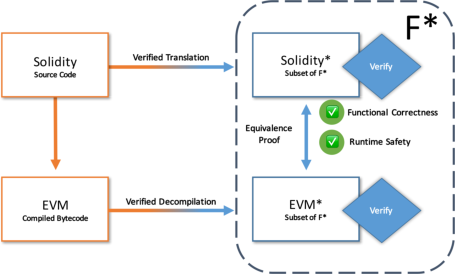
\includegraphics[width=0.6\textwidth]{./img/formal-verification-of-smart--contract.pdf}
\end{center}

\begin{block}{Disadvantages}
\begin{itemize}
\item Support only a fragment of EVM
\item No semantic argument for the translation
\item Code produced in hackathon not touched since
\end{itemize}
\end{block}
\end{frame}




\begin{frame}{Scilla}
\framesubtitle{\cite{scilla}}
\begin{block}{Smart Contract Intermediate Level LAnguage (WIP)}
\begin{enumerate}
\item Compile high-level language program (e.g., Solidity) to Scilla:
\begin{itemize}
\item Separation between computation and contract communication (e.g. communication last operation)
\end{itemize}
\item Conversion of Scilla in Coq (yet manually)
\item Mechanized Verification of properties (e.g., balance always $\geq 0$)
\item Compile Scilla to EVM bytecode
\end{enumerate}
\end{block}

\end{frame}


\begin{frame}{Static Analysis Tool}
% https://consensys.github.io/smart-contract-best-practices/security_tools/
\begin{block}{\href{https://github.com/trailofbits/manticore.git}{Manticore (Trail of Bits)}}
symbolic execution, taint analysis, and instrumentation to analyze binaries.
\end{block}
\begin{block}{\href{https://github.com/ConsenSys/mythril}{Mythrill (Consensys)}}
Concolic analysis, taint analysis and control flow checking to detect a variety of security vulnerabilities.
\end{block}


\end{frame}

\begin{frame}{Static Analysis Tool}


\begin{block}{SmartCheck~\cite{bib:smartcheck}}
\begin{itemize}
\item lexical and syntactical analysis on Solidity Source Code
\item Detect vulnerability patterns 
\item Show errors in source code
\item False positives because it cannot describe complex rules
\item No more activities since February 2018
\end{itemize}
\end{block}


\begin{block}{Solgraph}
Visualize Solidity control flow for smart contract security analysis
\begin{itemize}
\item Last release April 2017
\end{itemize}
\end{block}
\end{frame}





\begin{frame}{Open Challenges}
\begin{itemize}
\item Verified compilers~\cite{towardsVerifyingEthereumSmartContract}
\item Formalize semantics of Solidity code and
a compiler from Solidity into EVM, formally proving
is soundness against the formal semantics~\cite{grishchenko2018semantic}

\item Design an efficient static analysis  technique for EVM bytecode and to formally prove its soundness against the formal sematics~\cite{grishchenko2018semantic}

\item Optimize gas consumption in generated code~\cite{bib:gas}


\end{itemize}

\end{frame}







\begin{frame}[allowframebreaks]
        \frametitle{References}
        \bibliographystyle{apalike}
        \bibliography{bibliography.bib}
\end{frame}



\begin{frame}{EVM Alternative Languages}
\begin{block}{Bamboo~\cite{bamboo}}
\begin{itemize}
\item Polymorphic contracts: According to the stages, a contract changes its signature
\item Do not support loops
\end{itemize}
\end{block}

\begin{block}{Obsidian~\cite{obsidian}}
  \begin{itemize}
  \item State as first class citizen
  \item The methods that can be invoked on an object depend on the object’s current state.
  \end{itemize}
\end{block}
\end{frame}


\begin{frame}{Further tools}

\begin{block}{FSolidM~\cite{bib:FSolidM}}
\begin{itemize}
\item Generate solidity code from Final State Machine
\end{itemize}
\end{block}

\begin{block}{Dynamic Tools}
\href{https://github.com/sc-forks/solidity-coverage}{Solidity coverage}
\end{block}

\begin{block}{Linters}
\begin{itemize}
\item Solcheck
\item Solint
\item Solium
\item Solhint
\end{itemize}
\end{block}


\end{frame}



\end{document}

